% !TEX root=/home/tavant/these/manuscript/src/manuscript.tex

\section{Validation of the sheath model }
  \label{sec-sheath_validation}
  
  The \ac{PIC} simulations used here do not need any sheath model.
  In contrary, they can be used in order to validate the sheath modeled introduced in {\bf REF} coming from the fluid theory.
  This sheath model links the plasma potential drop with the electron temperature on the electron emission rate.
  The emission rate is linked to the electron temperature via \cref{eq-seemaxw}

  \Cref{eq-seemaxw} can be used to estimate the electron emission rate given the mean electron temperature measured in the simulations, corresponding statistically to the plasma bulk temperature.   
  
  In the \ac{PIC} simulations, \cref{eq-seeyield} can be computed by counting the number of electrons attaining the wall and emitted during a time-step.
  We note \ratepic this measurement.
   
  \begin{figure}[hbtp]
    \centering
    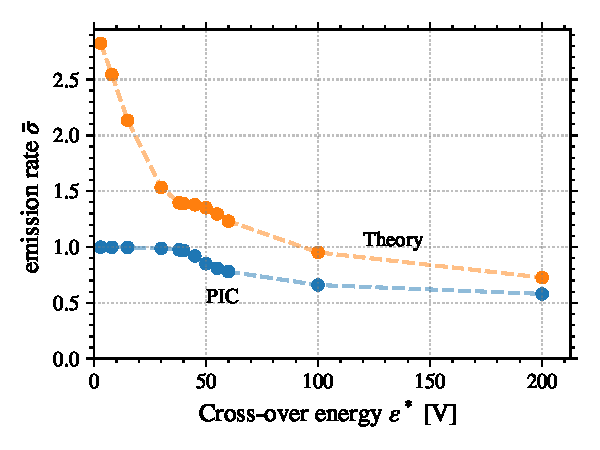
\includegraphics[width=\defaultwidth]{SEE_rates}
    \caption{Values of the electron emission rate $\rate$ (blue) measured in the simulation, and obtained with \cref{eq-seemaxw} using the electron temperature showed in \cref{fig-Tevsproba} }
    \label{fig-seeparamesMaxw}
  \end{figure}
  
  \begin{figure}[hbtp]
    \centering
    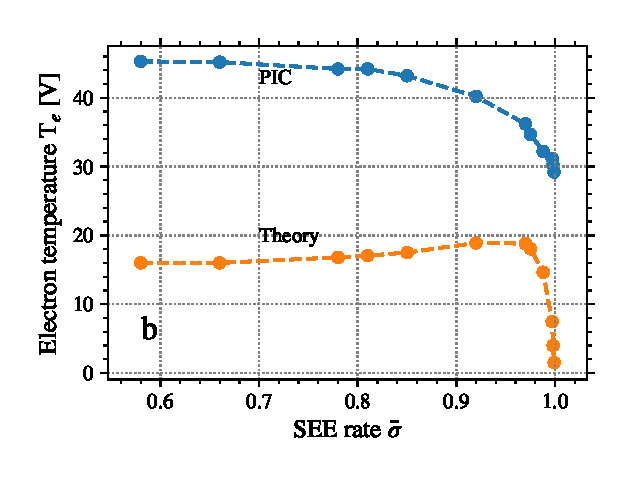
\includegraphics[width=\defaultwidth]{Te_pic_2}
    \caption{Mean electron temperature measured in the \ac{PIC} simulations as a function of the electron emission rate \rate, measured as well in the simulations.  }
    \label{fig-Tevsproba}
  \end{figure}
  
  
  We can see in \Cref{fig-seeparamesMaxw} that the mean electron emission rate lies between 0.6 for large $\crover$ and 1 at low $\crover$.
  The lower limit is expected, as $\proba_0 = 0.5$.
  On the other hand, the saturation of \ratepic at 1 was not expected.
  Indeed, \ratemaxw is equal to 2.9, and the electron temperature in the bulk measured, when, used in \cref{eq-seemaxw}, predicts a rate between 1.4 and 2.8.
  
  The electron temperature measured in the bulk of the simulation is presented in \cref{fig-Tevsproba} for the same cases as in \cref{fig-seeparamesMaxw}.
  We can see that when \rate increases, $\Te$ monotonically decreases from 45V to around 30V.
  However, these values do not explains the measured emission rate \ratepic.
    
  \begin{figure}[hbtp]
    \centering
    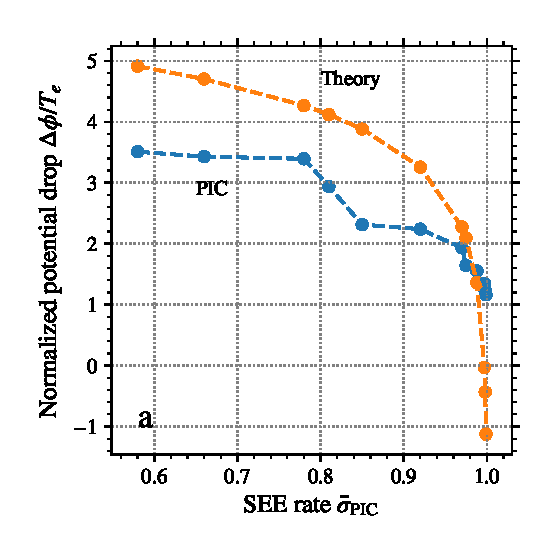
\includegraphics[width=\defaultwidth]{phi_drop_6}
    \caption{Plasma potential drop to the wall normalized by the electron bulk as a function of the electron rate. {\bf $\Te$ is italic !}}
    \label{fig-phi_rate}
  \end{figure}
  
  \Cref{fig-phi_rate} shows the evolution of the potential drop to the wall measured in the \ac{PIC} simulation compared to the theory \vref{eq-total_drop}.
  We see that at low emission rate, the potential drop is lower than expected.
  However, at high emission rate, the expected value tends toward negative values, while the measured values converges toward $\frac{\dphi}{\Te} = 1$.
  
  The sheath model of \cref{sec-sheath} used two hypotheses:
  \begin{itemize}
    \item Maxwellian electrons
    \item Isothermal evolution of the electrons
  \end{itemize}
  These two hypotheses will be confronted against the kinetic simulation in the next session.
  
  
   